\documentclass[final]{beamer}
\mode<presentation>
\usetheme{IWH}
% Use the beamerposter package
%\usepackage[orientation=portrait,size=a1,scale=1.15]{beamerposter}


\usepackage[orientation=portrait,scale=1.15]{beamerposter}
\setlength{\paperwidth}{36in}
\setlength{\paperheight}{48in}
\setlength{\textwidth}{0.98\paperwidth}
\setlength{\textheight}{0.98\paperheight}
\usepackage{graphicx} % for including images
\usepackage{amsmath} % for math symbols
\usepackage{amssymb} % for more math symbols
\usepackage{amsfonts}
\usepackage{lmodern} % scalable font package
\usepackage{booktabs}
\usepackage{colortbl}
\usepackage{multirow}
\usepackage{multicol}
\usepackage{subcaption}
\usepackage{setspace}

% Define poster colors and style
\usepackage{color}
\definecolor{darkblue}{rgb}{0.1,0.1,0.5}
\setbeamercolor{title}{fg=darkblue}

%\usepackage[pdftex,hiresbb]{graphicx}
%\usepackage[pageshow]{xtab}
\usepackage[bottom,hang,splitrule]{footmisc}
\usepackage[font={small},labelfont={bf},textfont={bf},format=hang,justification=RaggedRight]{caption}
\usepackage{tabularx}
\usepackage{natbib}
%\usepackage[spaces,hyphens]{url}
\usepackage{breakcites}
\usepackage{fancyhdr}
\usepackage{longtable}
\usepackage{dcolumn}
\usepackage{booktabs}
\usepackage{hyphenat}
%\usepackage[hidelinks]{hyperref}
\usepackage{doi}
\usepackage[UKenglish]{babel}
\usepackage[pdftex]{rotating} % [counterclockwise] %evtl. miteinbinden
\usepackage{color}
\usepackage[section]{placeins}
%\usepackage{subfig}
\usepackage{siunitx}
\sisetup{detect-all}


%%%%%%%%%%%%%%%5
\usepackage{environ}% Required for \NewEnviron, i.e. to read the whole body of the environment
\makeatletter

\newcounter{acolumn}%  Number of current column
\newlength{\acolumnmaxheight}%   Maximum column height


% `column` replacement to measure height
\newenvironment{@acolumn}[1]{%
	\stepcounter{acolumn}%
	\begin{lrbox}{\@tempboxa}%
		\begin{minipage}{#1}%
		}{%
		\end{minipage}
	\end{lrbox}
	\@tempdimc=\dimexpr\ht\@tempboxa+\dp\@tempboxa\relax
	% Save height of this column:
	\expandafter\xdef\csname acolumn@height@\roman{acolumn}\endcsname{\the\@tempdimc}%
	% Save maximum height
	\ifdim\@tempdimc>\acolumnmaxheight
	\global\acolumnmaxheight=\@tempdimc
	\fi
}

% `column` wrapper which sets the height beforehand
\newenvironment{@@acolumn}[1]{%
	\stepcounter{acolumn}%
	% The \autoheight macro contains a \vspace macro with the maximum height minus the natural column height
	\edef\autoheight{\noexpand\vspace*{\dimexpr\acolumnmaxheight-\csname acolumn@height@\roman{acolumn}\endcsname\relax}}%
	% Call original `column`:
	\orig@column{#1}%
}{%
	\endorig@column
}

% Save orignal `column` environment away
\let\orig@column\column
\let\endorig@column\endcolumn

% `columns` variant with automatic height adjustment
\NewEnviron{acolumns}[1][]{%
	% Init vars:
	\setcounter{acolumn}{0}%
	\setlength{\acolumnmaxheight}{0pt}%
	\def\autoheight{\vspace*{0pt}}%
	% Set `column` environment to special measuring environment
	\let\column\@acolumn
	\let\endcolumn\end@acolumn
	\BODY% measure heights
	% Reset counter for second processing round
	\setcounter{acolumn}{0}%
	% Set `column` environment to wrapper
	\let\column\@@acolumn
	\let\endcolumn\end@@acolumn
	% Finally process columns now for real
	\begin{columns}[#1]%
		\BODY
	\end{columns}%
}
\makeatother
%%%%%%%%%%

% Title, author, and date
\title{Smooth and Persistent Forecasts of German GDP}
%\subtitle[]{\hspace{1.9cm}\LARGE{ A quarterly evaluation of EU Commissions' GDP forecasts}}

\author[]{Katja Heinisch$^{\textit{ 1}}$, Simon van Norden$^{\textit{ 2}}$, Marc Wildi$^{\textit{ 3}}$}
\institute[IWH]{\normalsize{$^{\textit{1}}$ Halle Institute for Economic Research (IWH), $^{\textit{2}}$ HEC Montréal and CIREQ, $^{\textit{3}}$ Zurich University of Applied Sciences (ZHAW) }}
%\author[]{Katja Heinisch}
%\institute[IWH]{Halle Institute for Economic Research}
%\vspace{2cm}


\begin{document}
	
	\begin{frame}
		\begin{columns}[T]
			% Column 1
			\begin{column}{0.48\textwidth}
					\begin{block}{\large Motivation}
								
					\begin{itemize}
					\item Forecasting dilemma: Efficiency requires full use of information, yet resulting forecasts are often highly volatile.
				%	Trade-off between informational efficiency and forecast smoothness.
					\item Short-term volatility and data revisions challenge reliable forecasting.
				\item \cite{Wildi2024,Wildi2025,McElroy2019,McElroy2020} propose the Smooth Sign Accuracy (SSA) framework, which controls volatility via penalizing forecast sign changes.
				\\
				\vspace{1cm}
					 {\textbf{\textcolor{iwhdarkblue}Research Questions:}}
			
					\item Can we improve GDP forecast smoothness without sacrificing accuracy?
					\item Do multivariate filtering techniques enhance persistence and coherence?
					\\
					$\rightarrow$ 	We propose methods to produce smooth and persistent forecasts of German GDP, i.e. by replacing raw leading indicators with smoothed and filtered components derived from the M-SSA procedure, thereby improving the signal-to-noise ratio in the predictor variables used to forecast GDP in the mid of a particular quarter.
					\end{itemize}
			
			\end{block}
					
		\begin{block}{\large Data}
															
					  \begin{columns}[T]
						\column{0.495\textwidth}
							\begin{itemize}
							     \item Quarterly German GDP (1995–2024).
							     \item Monthly Indicators: Industrial Production, ifo Business Climate, ESI, Term spread 10y-3m.
							     \item Log-differenced, standardized (except spreads), outliers trimmed ( COVID-19).
							     \item Data aligned to account for publication lags and converted to quarterly frequency 
							     \item Dynamic dependencies are explored via cross-correlation functions (CCFs) and vector moving-average (VMA) representations.
							     \item Survey indicators show strong leading correlations with GDP; IP and term spread exhibit weaker or delayed effects.
							     \item Pandemic-related outliers distort dynamic patterns; hence, data from Q4-2019 to Q4-2020 are excluded for stability.
							\end{itemize}
								   							  	
						\column{0.495\textwidth}
									\begin{center}
										{\small{\textbf{\textcolor{black}{Figure 1: Leads \& lags}}}}
									
									    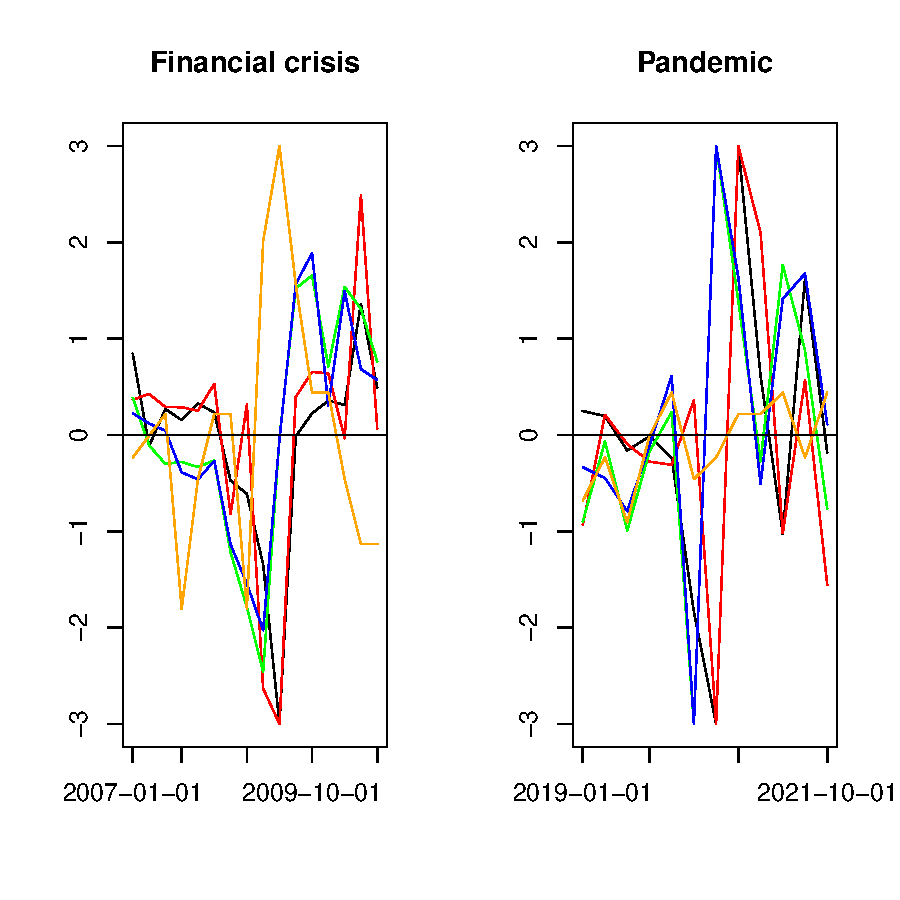
\includegraphics[width=1\textwidth]{./Figures/data_lags.pdf}
									\end{center}

								\leftskip2em \singlespacing{ {\footnotesize \emph{Note:} GDP \& Indicators: standardized log-differences, trimmed to $\pm 3$ standard deviations.} }
						\end{columns}
				
			
					
				\end{block}
				
		\begin{block}{\large{Direct Forecasts}}
			\begin{itemize}
				\item Regression of GDP on contemporaneous indicators, i.e. VARMA dynamics estimated via parsimonious VAR(1).
				\item Impulse responses reveal GDP reacts most strongly to survey shocks, with modest delayed response to IP.
				\item These dynamics motivate the use of multivariate models to improve forecast accuracy beyond univariate benchmarks.
				\item The results indicate that as the forecast horizon $h$ increases, the turning points (i.e., peaks and troughs) of the direct forecasts become increasingly right-shifted (lagged) relative to the target GDP. 
			\end{itemize}
		
		\begin{columns}[T]
			\column{0.495\textwidth}
									
				\textcolor{iwhdarkblue}{\textbf{Filtering Indicators}}
					\begin{itemize}
						\item Forecasts are re-estimated using indicators smoothed via the one-sided HP-C filter (HP(160)).
						\item Figures show improved alignment: forecasts lag GDP less and better capture turning points.
						\item Filtering reduces high-frequency noise and enhances signal extraction.
					\end{itemize}
				\begin{footnotesize}
						\begin{table}[h]
						\begin{center}
								{\small{\textbf{\textcolor{black}{Table 1: }}}}
						\begin{tabular}{lrrrrrrr}
							\hline
							& h= 0 & h= 1 & h= 2 & h= 3 & h= 4 & h= 5 & h= 6 \\ 
							\hline
							Unfiltered & 0.028 & 0.000 & 0.001 & 0.910 & 0.509 & 0.091 & 0.178 \\ 
							HP-C filtered & 0.000 & 0.001 & 0.036 & 0.046 & 0.049 & 0.012 & 0.022 \\ 
							\hline
						\end{tabular}
						\leftskip2em \singlespacing{ {\footnotesize \emph{Note:} p-values for $H_0: \hat{\beta} = 0$, HAC-adjusted Wald test.\\Estimation over full sample (without pandemic.)					\label{tab:pvaluedhp}}}
						\end{center}
						\end{table}
				\end{footnotesize}
			\begin{itemize}
				\item HP-C filter improves smoothness but remains univariate and prone to high-frequency leakage.
			\end{itemize}
		
			
				\column{0.495\textwidth}
									
				\begin{center}
				{\small{\textbf{\textcolor{black}{Figure 2: Performance of direct forecasts}}}}
				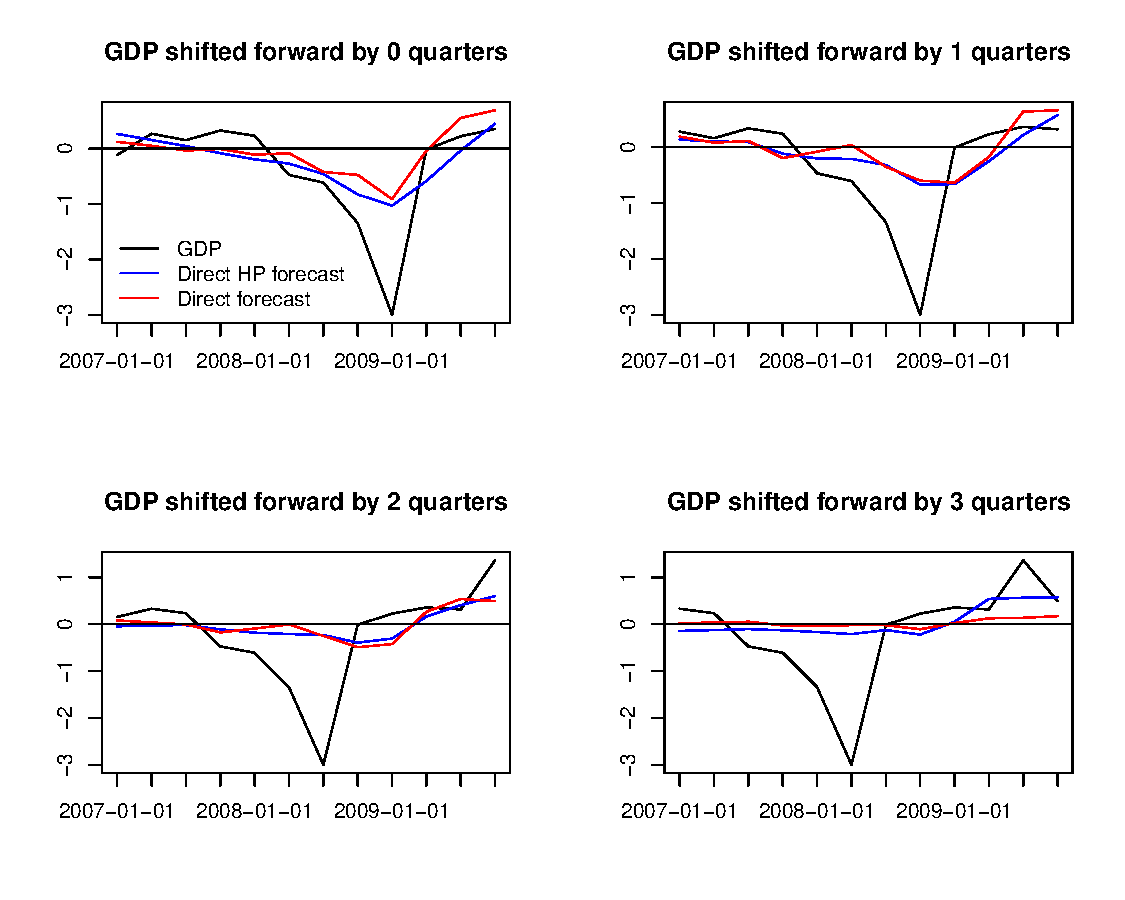
\includegraphics[width=1\textwidth]{./Figures/direct_hp_forecasts_financial_crisis.pdf}
				\end{center}
			
				\end{columns}	
			\end{block}		
			
				\begin{block}{\large Empirical Approach -- Multivariate Smooth Sign Accuracy (M-SSA)}
						\addtolength{\itemsep}{10pt}
			%	\textcolor{iwhdarkblue}{\textbf{Filtering Indicators}}
            \begin{columns}[T]
			\column{0.495\textwidth}
            
				\begin{itemize}
				 
				\item M-SSA extends SSA (\cite{Wildi2025}) to multivariate setting with causal (one-sided) filters.
				\item Target variable $z_t$ (e.g. HP-GDP) is tracked by predictor $y_t$ via multivariate filters on leading indicators.
				\item SSA criterion: maximize forecast-target correlation under constraint on forecast autocorrelation $\rho(y,1)$.
				\item Constraint controls smoothness via expected holding time: $ht(y) = \frac{\pi}{\arccos(\rho(y,1))}$.
				\item Optimization via constraints on sign-changes.
			\end{itemize}
            \column{0.495\textwidth}
									
				\begin{center}
				{\small{\textbf{\textcolor{black}{Figure 3: M-SSA vs. HP-C}}}}
				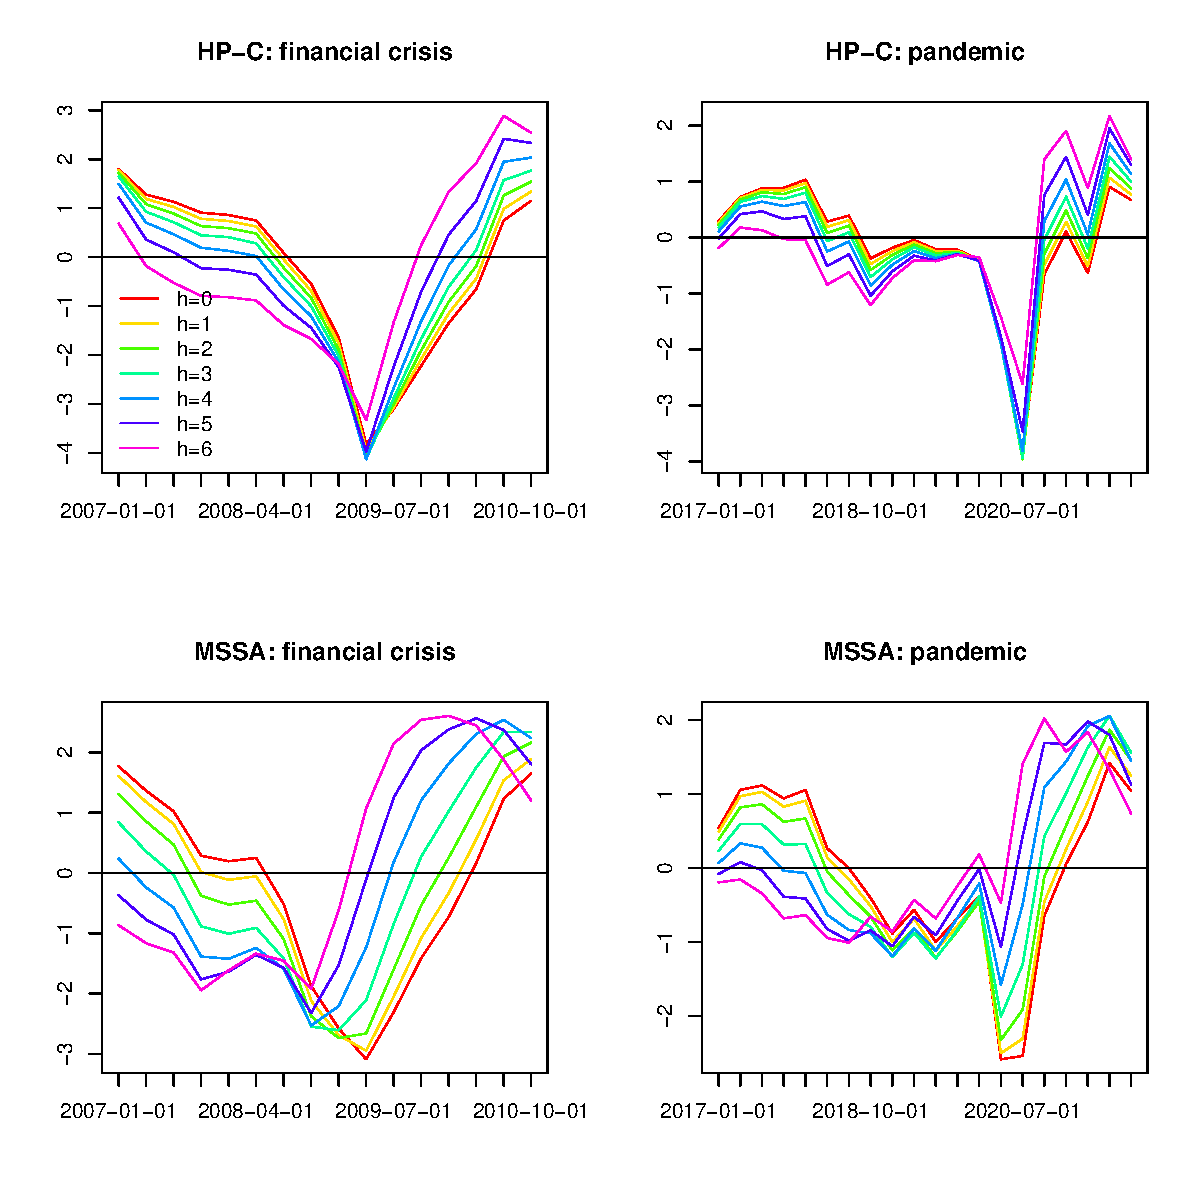
\includegraphics[width=1\textwidth]{./Figures/multivar_vs_univar.pdf}
				\end{center}
			
				\end{columns}	
            
%	\autoheight
			\end{block}
				
			\end{column}
		%%%%%%%%%%%%%%%%%%%%%%%%%%%%%%%%%%%%%%%%%%%%%%%%%%%%%%
			% Column 2
		\begin{column}{0.48\textwidth}
			
			\begin{block}{\large{Results}}
				
			\begin{columns}
			\column{0.495\textwidth}
			\textcolor{iwhdarkblue}{\textbf{M-SSA Nowcasts vs M-MSE}}\\
			\begin{itemize}
			\item Comparison of nowcasts for HP-GDP using M-SSA vs M-MSE.
			\item M-SSA reduces sign changes by 33\% with minimal loss of accuracy.
			\item M-SSA achieves longer holding times: a $50\%$ increase compared to M-MSE
			\end{itemize}
		
		\column{0.495\textwidth}
			  \begin{center}
			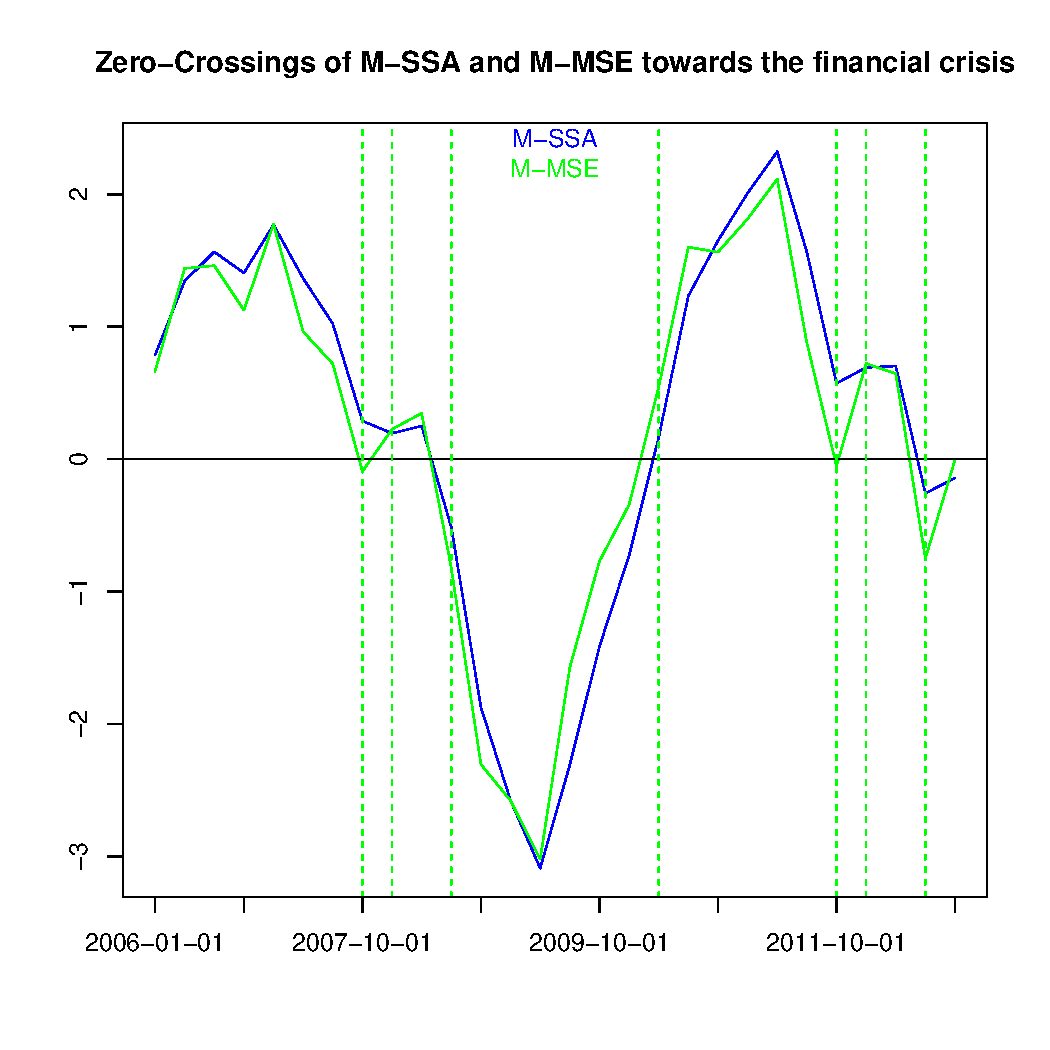
\includegraphics[width=0.8\textwidth]{./Figures/mssa_msse_zc.pdf}
				\leftskip2em \singlespacing{ {\footnotesize \emph{Note:}{Two-sided HP(160) applied to GDP (black)\\ Nowcasts: M-SSA (blue) and M-MSE (green). \\The dashed vertical line delimits in- and out-of sample periods.  \\The two-sided filter does not extend to the sample end.
				\label{mssa_msse_now}}}}
		\end{center}
		\end{columns}
		
		
					\vspace{0.5cm}
					\textcolor{iwhdarkblue}{\textbf{M-SSA Forecasts for $h > 0$}}\\
					
						\begin{itemize}	
								\addtolength{\itemsep}{10pt}	
					\item As the forecast horizon hh increases, M-SSA filter weights decrease, indicating greater uncertainty.
					\item M-SSA forecasts shift leftward consistently as $h$ increases, especially around turning points.
	
						\end{itemize}	
				
			\vspace{0.5cm}
			
			\textcolor{iwhdarkblue}{\textbf{M-SSA Component Predictor}}\\
				\begin{itemize}
				\item M-SSA components, derived from HP(160)-filtered indicators, are used as predictors for unfiltered GDP via a post-processing regression step.
				\item The M-SSA filters are fixed using data up to January 2008, while component weights are updated quarterly using an expanding window starting from January 2008.
				\item A linear regression maps the M-SSA output at horizon $h$ to forward-shifted GDP at $t + \text{shift}$, correcting for scaling and allowing for $h \neq \text{shift}$.
				\item This setup enables leveraging the forecast-leading behavior (left-shift) of M-SSA predictors, particularly when $\text{shift} < h$.
			\end{itemize}
			\begin{columns}
					\column{0.495\textwidth}
				
			\begin{itemize}
			\item Out-of-sample forecast performance is evaluated by comparing the M-SSA-based predictor to both a mean forecast and a direct forecast, all updated quarterly.
			\item Results show that for longer horizons ($h \geq 4$), M-SSA predictors outperform both benchmarks, especially at shorter shifts, confirming the predictive value of their anticipatory signal.
			\item Statistical significance of the M-SSA GDP predictor is confirmed for up to one year ahead, excluding the pandemic period.
			\end{itemize}
		
		
			\column{0.495\textwidth}
\begin{table}[ht]
	\centering
			{\small{\textbf{\textcolor{black}{Table 2: rRMSEs }}}}\\
\begin{footnotesize}
	\begin{tabular}{rrrrrrrr}
		\hline
		& h=0 & h=1 & h=2 & h=3 & h=4 & h=5 & h=6 \\ 
		\hline
		Shift=0 & 0.978 & 0.942 & 0.893 & 0.855 & 0.860 & 0.906 & 0.962 \\ 
		Shift=1 & 1.082 & 1.060 & 1.005 & 0.926 & 0.877 & 0.880 & 0.914 \\ 
		Shift=2 & 1.083 & 1.090 & 1.077 & 1.019 & 0.952 & 0.918 & 0.919 \\ 
		Shift=3 & 1.034 & 1.059 & 1.081 & 1.063 & 1.010 & 0.970 & 0.954 \\ 
		Shift=4 & 0.995 & 1.029 & 1.069 & 1.077 & 1.035 & 0.986 & 0.953 \\ 
		Shift=5 & 0.993 & 1.030 & 1.075 & 1.093 & 1.062 & 1.011 & 0.967 \\ 
		\hline
	\end{tabular}
\end{footnotesize}
\begin{singlespace}
	{\footnotesize \emph{Notes:} : Out-of-sample forecast errors  vs expanding mean forecast of GDP. Out-of-sample evaluation starting in Q1 2008, without pandemic.\\Values $< 1$ indicate superior predictions.}
\end{singlespace}
\vspace{0.5cm}
\end{table}
\end{columns}

\vspace{0.5cm}
\textcolor{iwhdarkblue}{\textbf{Receiver Operating Characteristic (ROC)}}\\
   
\begin{columns}
    \column{0.495\textwidth}
      \begin{itemize}
			\item Compute sign accuracy and false positive rate: ROC curves
            \item Compute Area Under Curve (AUC)
			\item All filters outperform direct forecast (larger AUC) for $h>2$ 
			\end{itemize}



\begin{table}[ht]
	\centering
			{\small{\textbf{\textcolor{black}{Table 3: AUCs }}}}\\
\begin{footnotesize}
\begin{tabular}{rrrrr}
  \hline
 & Direct & HP-C & M-MSE & M-SSA \\ 
  \hline
Forecast horizon 1 & 0.752 & 0.715 & 0.746 & 0.747 \\ 
  Forecast horizon 2 & 0.697 & 0.663 & 0.729 & 0.720 \\ 
  Forecast horizon 3 & 0.554 & 0.622 & 0.684 & 0.709 \\ 
  Forecast horizon 4 & 0.486 & 0.624 & 0.680 & 0.708 \\ 
  Forecast horizon 5 & 0.593 & 0.636 & 0.643 & 0.701 \\ 
   \hline
\end{tabular}
\end{footnotesize}
\begin{singlespace}
	{\footnotesize \emph{Notes:} :AUCs of predictors against GDP at various forecast horizons.}
\end{singlespace}
\vspace{0.5cm}
\end{table}

    \column{0.495\textwidth}
        \begin{center}
        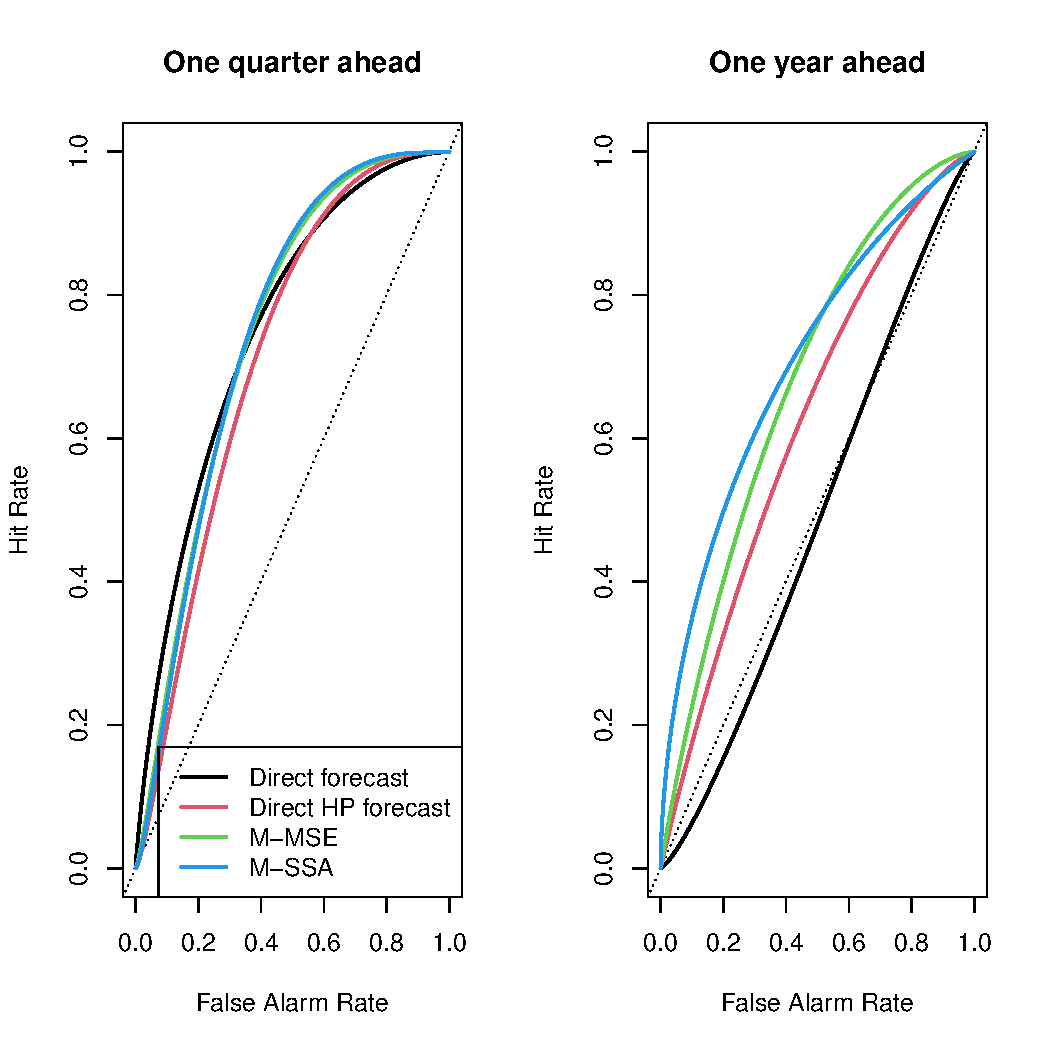
\includegraphics[width=0.8\textwidth]{./Figures/ROC_GDP_shift_1_4.pdf}
		
	     \end{center}
    
\end{columns}
   
			
			\end{block}
			
			\begin{block}{\large Summary and Conclusion}
				
			\begin{itemize}
            \item Classic direct forecasts of GDP perform well up to two quarters ahead but suffer from noise and limited horizon; smoothing with an HP(160)-filter improves performance during sharp recessions yet retains some noise-induced sign changes.
            \item To overcome these limitations, a multivariate SSA (M-SSA) framework based on \cite{Wildi2024} is introduced, leveraging cross-sectional indicator data and controlling the predictor’s zero-crossing rate for enhanced signal tracking at turning points.
            \item A simple regression of the M-SSA GDP component on future GDP yields a statistically significant predictor up to one year ahead, outperforming both mean benchmarks and classic direct forecasts at longer horizons.
            \item Stability in regression coefficients and filter design after a burn-in period improves the interpretability of the predictor, offering a robust integration of direct forecasting with multivariate signal extraction targeting quarterly GDP growth.
        \end{itemize}
			\end{block}
			
	
	
	\begin{block}{\large References and Further Information}
	\begin{columns}[T]
		\column{0.3\textwidth}
		

		\column{0.5\textwidth}
				%\begin{flushright}	
                GIT: https://github.com/wiaidp/R-package-SSA-Predictor
				%\end{flushright}
				\column{0.2\textwidth}

			%\includegraphics[width = 0.55\textwidth]{../Figures/GIT.pdf}
		\end{columns}

	\end{block}
		\end{column}
	\bibliographystyle{apalike}
	\bibliography{references}
\end{columns}

\end{frame}

\end{document}
